\section{Motivation}
\label{sec:motivation}

In diesem Versuch geht es darum, mit Hilfe des optischen Pumpens den
Kernspin zweier Rubidium Isotope zu bestimmen. Dazu wird ein Gasgemisch
der Isotope mit HF\footnote{Hochfrequenz}-Strahlung bestrahlt um durch
das herstellen einer Besetzungsinversion letztendlich auf den Kernspin
zu schließen.

\section{Theoretische Grundlagen}
\label{sec:theorie}

\subsection{Energieniveaus der Rubidiumisotope}

Rubidium ist ein Alkalimetall, welches nur ein Elektron in der fünften Schale hat.
Die Quantenzahl der Elektronenhülle hängt also ausschließlich von diesem Elektron ab.
Bei Vernachlässigung jeglicher Korrekturen liegt das Elektron als Spin-1/2-Teilchen
in dem Zustand mit $n=5$, $L=0$ und $M_L=0$, wobei $n$ die Hauptquantenzahl,
$L$ die Neben- oder auch Drehimpulsquantenzahl und $M_L$ die zu ihr
gehörige magnetische Quantenzahl bezeichnet.
In niedrigster Ordnung verfügt das Niveau mit $L=1$ und $M_L=0,\pm1$
über die gleiche Energie wie der besetzte Zustand, sie sind also entartet.

In nächster Näherung wird die Spin-Bahn-Kopplung betrachtet welche zeigt,
dass die obige Entartung nicht korrekt sein kann.
Eine neue Erhaltungsgröße $J$, welche aus der Vektoraddition
des Bahndrehimpulses $\vec{L}$ und des Spins $\vec{S}$ des Elektrons besteht, ist der Grund.
Die neuen Quantenzahlen $J$ und $M_J$ definieren nun einen Zustand,
wobei $J$ von $\lvert L - S \rvert$ bis $\lvert L + S \rvert$ geht.
Somit sind Zustände mit unterschiedlichem $J$ nicht mehr entartet,
jedoch bleibt die $M_J$ Entartung ohne äußeres $B$-Feld erhalten.
Diese Aufspaltung wird auch Feinstruktur genannt.

\begin{figure}
    \centering
    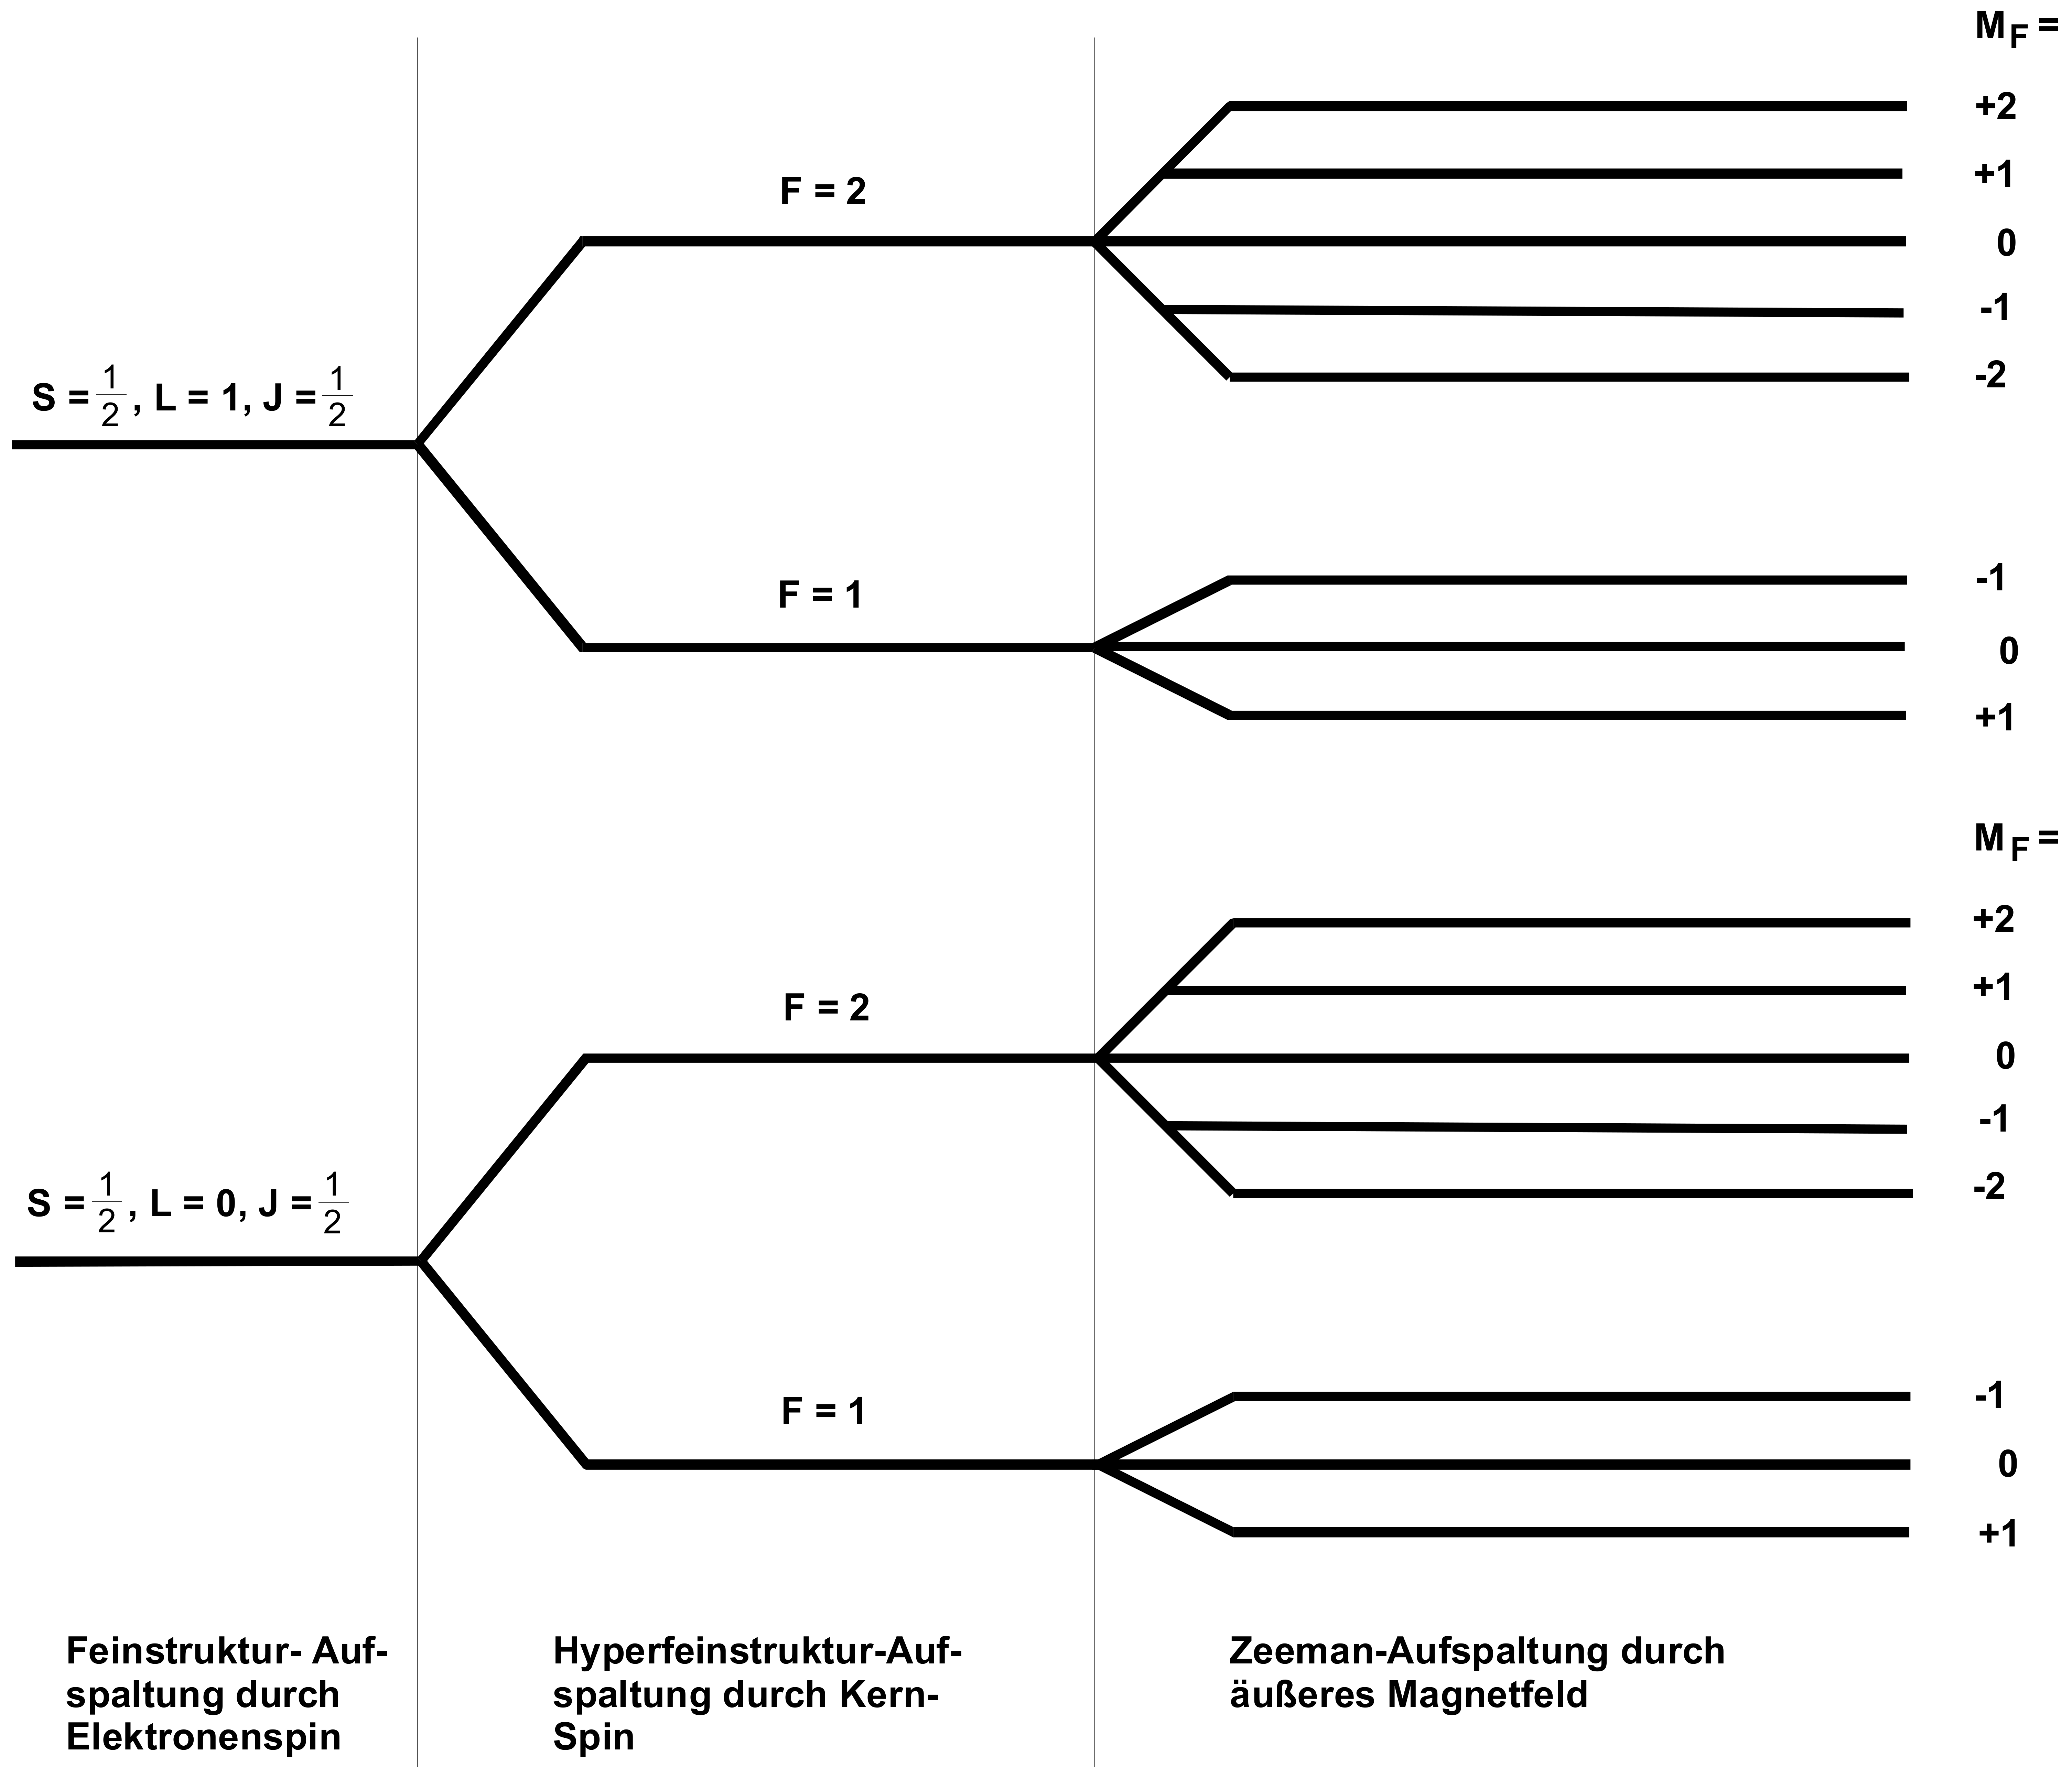
\includegraphics[width=0.7\textwidth]{images/feinstruktur.png}
    \caption{Schematische Darstellung der Energieniveaus in \ce{^{87}Rb} mit $I=3/2$ \cite{anleitungAlt}.}
    \label{fig:energyN}
\end{figure}

Die nächste Korrektur erhält man nun, wenn die Spin-Spin-Kopplung des Gesamtdrehimpulses
der Elektronenhüllen an den Kernspin betrachtet wird.
Der Gesamtimpuls $\vec{F}$ setzt sich aus der Vektoraddition von $J$ und $I$.
$F$ kann Werte zwischen $\lvert J - I \rvert$ und $\lvert J + I \rvert$ annehmen,
mit $M_F$ als magnetischer Quantenzahl.
Ohne äußeres Magnetfeld bleiben Zustände mit verschiedenem $M_F$ trotz gleichen $F$
entartet.

Für die Aufhebung dieser Entartung ist der Zeeman-Effekt verantwortlich.
Er spaltet einen $F$\;Zustand in $2F$+1-Zustände auf.
Die Energiedifferenz zweier benachbarter Zeeman-Niveaus beträgt

\begin{equation}
  \Delta E_Z = g_F \mu_{\text{B}} B
  \label{eqn:zeemanDifferenz}
\end{equation}

und ist somit proportional zur magnetischen Flussdichte $B$.
Der Faktor $\mu_{\text{B}} = \frac{e \hbar}{2m_e}$ ist das Bohrsche Magneton,
das kleinstmögliche magnetische Moment welches ein Elektron tragen kann.
Der Landé-Faktor des Gesamtdrehimpulses des Atoms $g_F$ ergibt sich aus
Kopplungsdiagrammen der beteiligten Drehimpulse näherungsweise zu
\begin{equation}
  g_F = g_J \frac{F(F+1)+J(J+1)-I(I+1)}{2F(F+1)}\,,
  \label{eqn:g_F_Theorie}
\end{equation}
wobei der Landé-Faktor des Gesamtdrehimpulses des Elektrons
\begin{equation}
  g_J = \frac{3{,}0023J(J+1)+1{,}0023(S(S+1)-L(L+1))}{2J(J+1)}
  \label{eqn:g_J_Theorie}
\end{equation}
beträgt.

\subsection{HF-Spektroskopie und das Prinzip des optischen Pumpens}
\label{subsec:opticalPump}

Die häufig verwendete Schreibweise für die Darstellung der Feinstrukturniveaus
ist ${}^{2S+1}L_J$ mit der Multiplizität $2S+1$ und dem Kennbuchstaben $L$ für den
elektronischen Drehimpuls, wobei $L=0,1,2,...$ den Schalen $S,P,D,...$ zugeordnet wird.
Ohne äußere, zeitabhängige Störung folgt die Besetzung dann näherungsweise einer thermischen Boltzmann-Verteilung,
sodass die Elektronen größtenteils im Grundzustand mit niedrigstem $m_F$ sind.
Es wird nun rechtszirkular polarisiertes Licht der Frequenz des $D_1$-Überganges eingestrahlt, dessen Energie dem
Übergang von ${}^{2}P_{1/2}$ nach ${}^{2}S_{1/2}$ entspricht. Übergänge, die durch Absorption dieser Photonen
entstehen, gehorchen der Auswahlregel $M_F=+1$, während die spontane Emission keine bestimmten Übergänge
bevorzugt. Es gelingt also, durch dieses Prinzip den niedrigsten Zustand nahezu leer zu pumpen und den
$S$-Zustand mit $F=2$, $M_F=2$ anzureichern und eine Besetzungsinversion herbeizuführen.
Eine schematische Darstellung der erlaubten übergänge bei einem Pumpvorgang sind in Abbildung \ref{fig:pumping}
dargestellt.

\begin{figure}
    \centering
    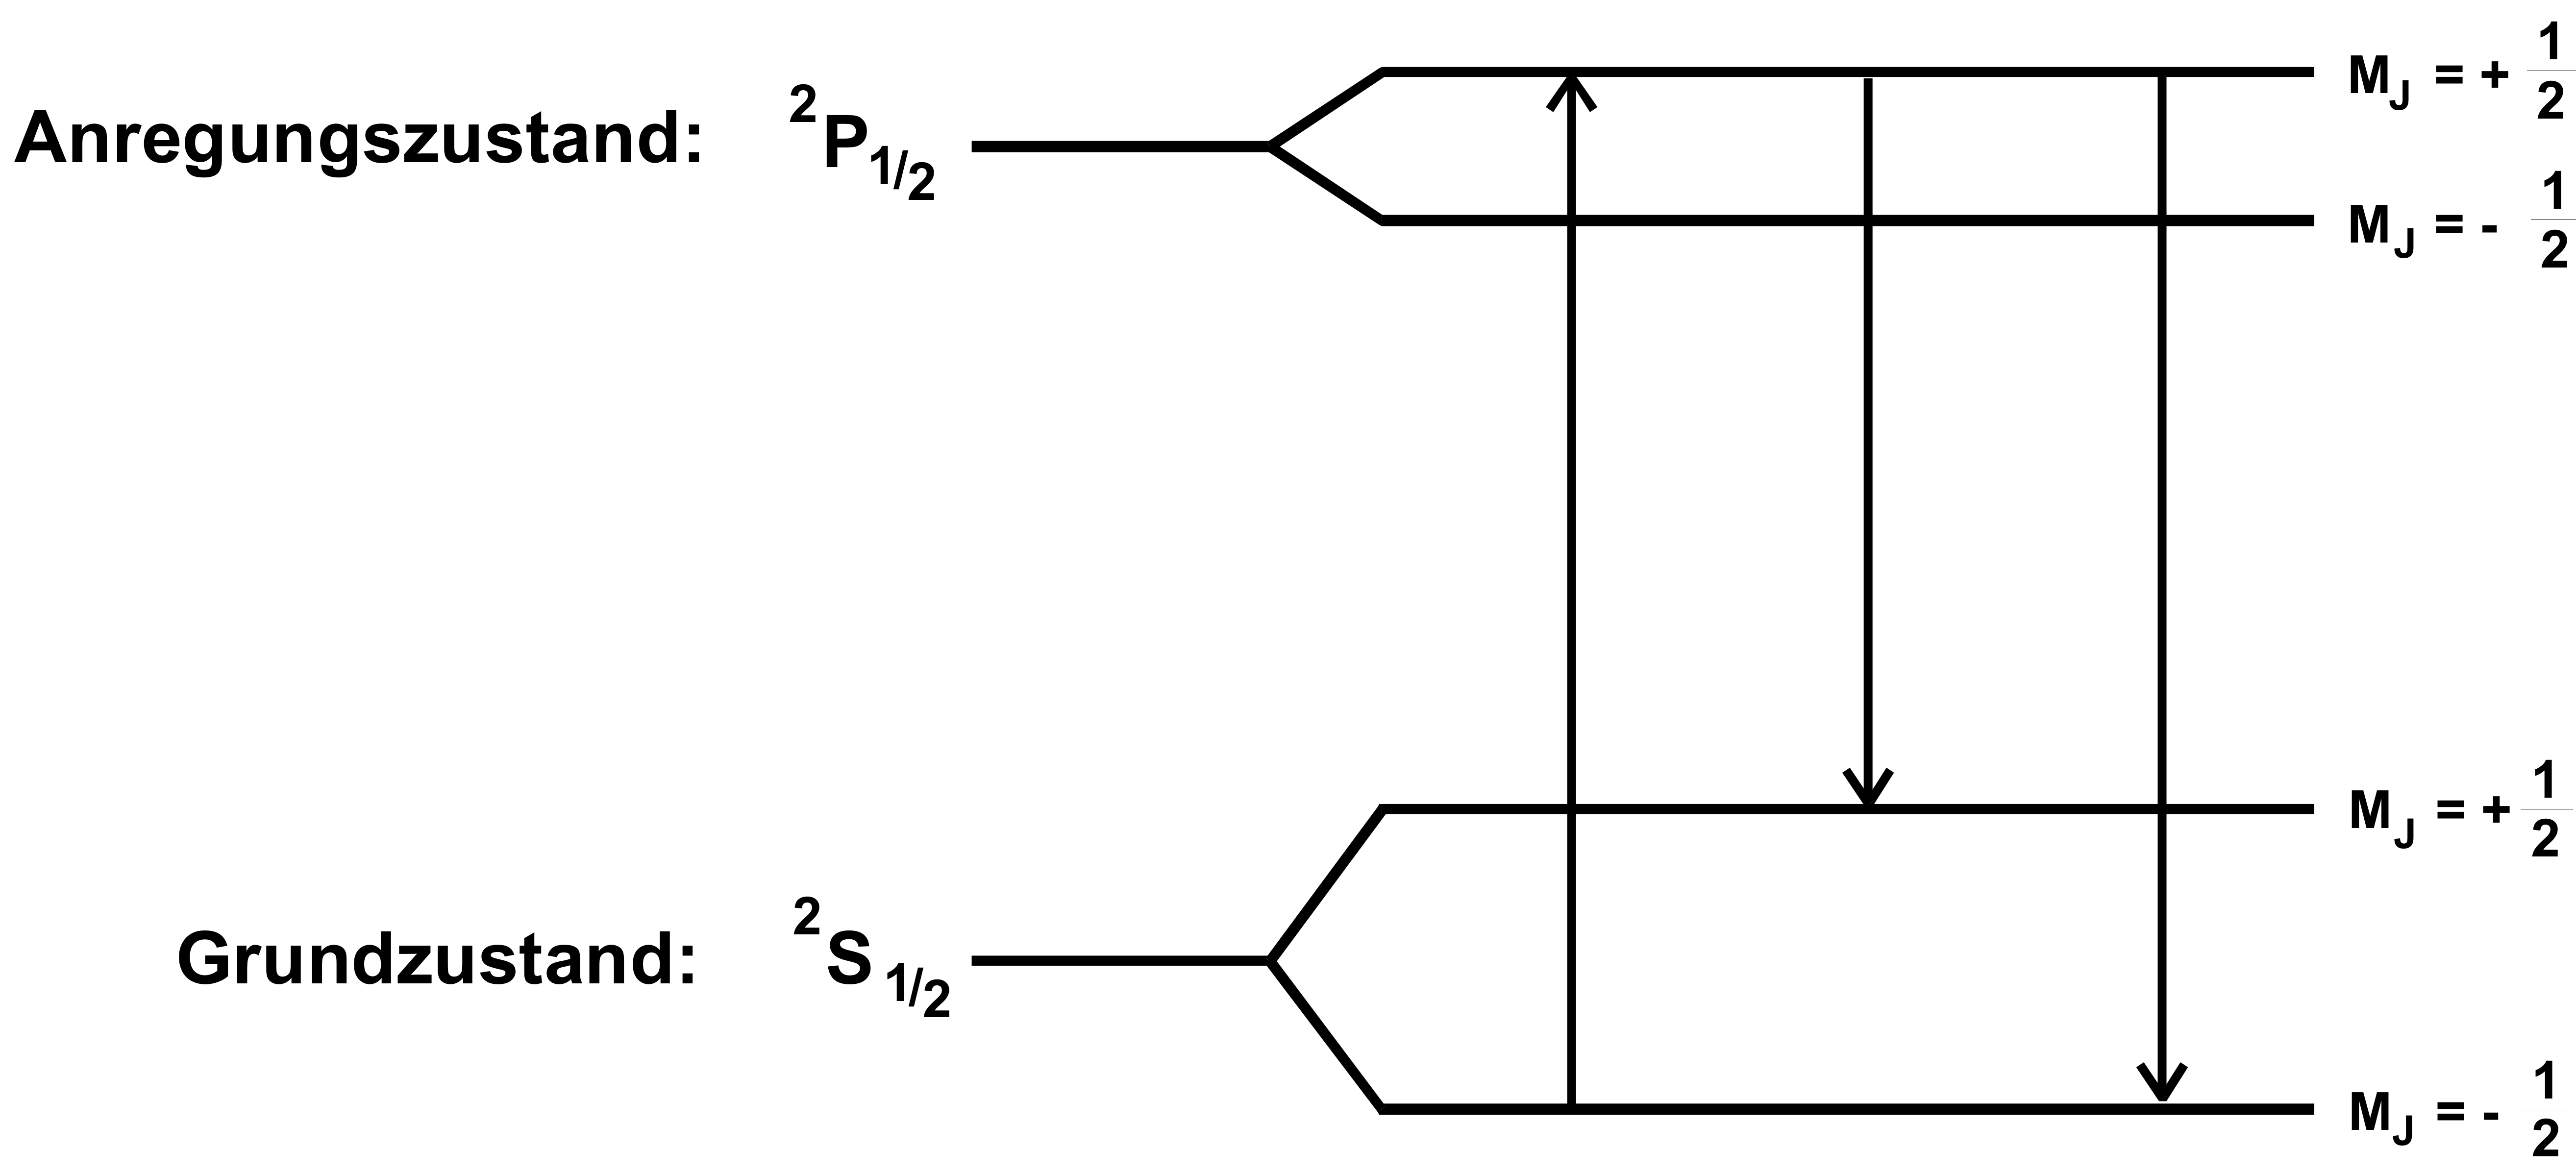
\includegraphics[width=0.7\textwidth]{images/rechtszirkulareEinstrahlung.png}
    \caption{Schema des Pumpvorgangs für Rubidiumatome bei Einstrahlung von rechtszirkular polarisiertem Licht. \cite{anleitungAlt}}
    \label{fig:pumping}
\end{figure}

Ein geeignetes Maß für die Besetzungsinversion stellt die Transparenz der Dampfzelle gegenüber dem
einstrahlenden $D_1$-Licht dar. Diese wird mit einer ansteigenden Exponentialfunktion parametrisiert,
welche sich bei vollständiger Inversion sättigt, da das Licht dann aufgrund der Auswahlregel keinen
Übergang anregen kann. Obwohl die Zeeman-Aufspaltung das Phänomen des optischen Pumpens erst möglich
macht, wird Letzteres oft als spektroskopisches Verfahren eingesetzt, um die aufgespaltenen
Energieniveaus mit hoher Genauigkeit zu vermessen. Dieses Messverfahren bedient sich eines zweiten,
hochfrequenten magnetischen Feldes (RF-Feld), welches stimulierte Emission aus den angereicherten
Niveau heraus anregt. Für die Flussdichte $B_m$ gilt dann

\begin{equation}
  h f = g_F \, \mu_{\text{B}} B_m \Delta M_F \implies B_m = \frac{4 \pi m_e}{e g_F} f\,,
  \label{eqn:B_M_Theorie}
\end{equation}

sodass ein linearer Zusammenhang zu der Frequenz des Feldes besteht.
Da mit der stimulierten Emission eine Entleerung des zuvor angereicherten Niveaus verbunden wird, wird das Erreichen
der Feldstärke $B_m$ mit einer deutlichen Abnahme der Transparenz des Gases verbunden sein, weil der konkurrierende
Prozess der Besetzungsinversion durch optisches Pumpen wieder aufnehmen kann. Grafisch ist dies in Abbildung
\ref{fig:transparenz} dargestellt. Der ausgedehnte Dip um Null herum ist dem Erdmagnetfeld zuzuschreiben, während
der $B_m$-Dip durch das resonante RF-Feld bewirkt wird.

\begin{figure}
  \centering
  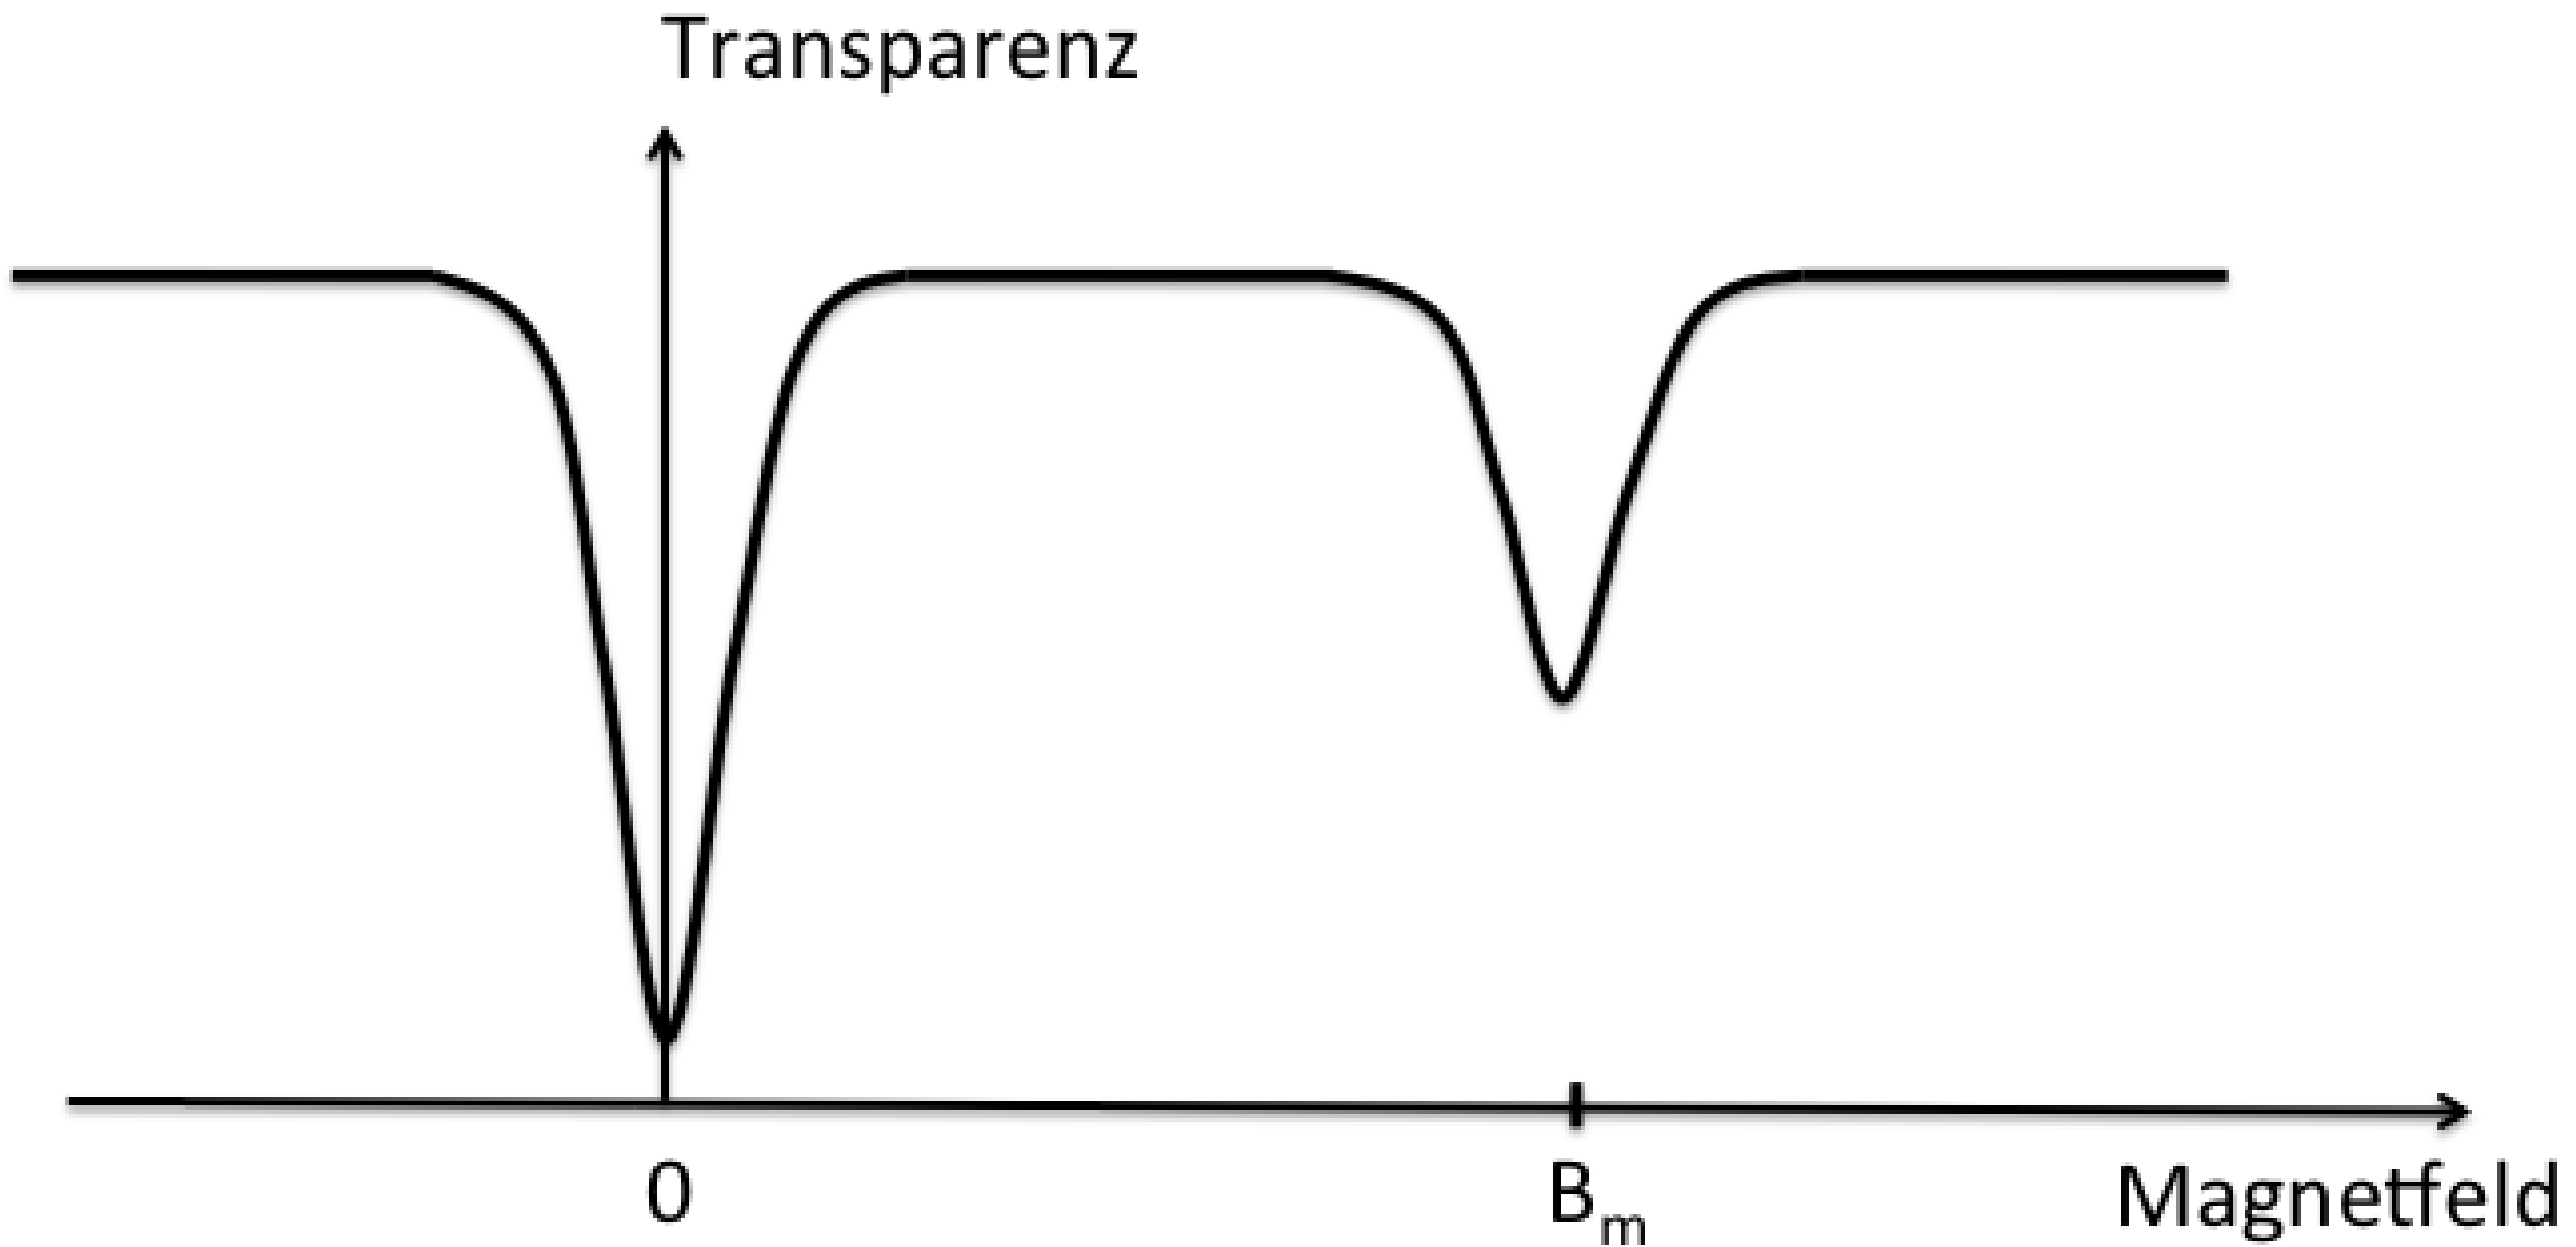
\includegraphics[width=0.6\textwidth]{images/transparenz.png}
  \caption{Transparenz der Dampfzelle in Abhängigkeit eines äußeren Magnetfelds.
          \cite{anleitung}}
  \label{fig:transparenz}
\end{figure}

Um 0 herum sinkt die Transparenz deutlich ab, dort kann keine Besetzungsinversion hergestellt werden. Dies liegt
daran, dass dies in einem Zweiniveausystem nicht möglich ist, da die Prozesse der Absorption und der
stimulierten Emission miteinander konkurrieren, wobei die zusätzliche spontane Emission die Besetzung des
Grundzustandes noch weiter bevorzugt. Experimentell wird dies ausgenutzt, um den Einfluss des Erdmagnetfelds zu minimieren.

\subsection{Der quadratische Zeeman-Effekt}
\label{subsec:quadratischerZeeman}

Bei schwachen Magnetfeldern können die obigen Annahmen getroffen werden.
Sobald starke Felder angelegt werden, wird die Drehimpulskopplung getroffen.
Um die Effekte bei mittleren Feldern zu untersuchen, werden zusätzliche
Terme der Störungsreihe in Betracht gezogen. Hierbei spricht man unter anderem vom
quadratischen Zeeman-Effekt. In niedrigster Ordnung kann die Energiedifferenz
aus Gleichung \eqref{eqn:zeemanDifferenz} zu

\begin{equation}
  \Delta E_Z = g_F \, \mu_{\text{B}} B + g_F^2 \, \mu_{\text{B}}^2 B^2 \frac{1-2M_F}{\Delta E_{\text{Hy}}}
  \label{eqn:zeequadr}
\end{equation}

korrigiert wird, wobei $E_\text{Hy}$ die Hyperfeinstrukturaufspaltung zwischen den
Niveaus $F$ und $F+1$ bezeichnet.


\subsection{Magnetfeld im Mittelpunkt einer \textsc{Helmholtz}-Spule}
Die Magnetfelder werden in diesem Versuchsaufbau mit \textsc{Helmholtz}-Spulen erzeugt.
Die Stärke des Magnetfeldes $B$ im Mittelpunkt kann ausgehend vom
\textsc{Biot}-\textsc{Savart}-Gesetz
\begin{align}
  B_i\l(x\r) &= \frac{μ_o n_i I_i R_i}{2\l(R_i^2 + x^2\r)^{\frac{3}{2}}}
  \shortintertext{als}
  B &= \left(\frac{4}{5}\right)^{\frac{3}{2}} \frac{μ_0 n I}{R}
  \label{eqn:helmholtz}
\end{align}
bestimmt werden.
